\section{Introduction}
\label{sec:coral-island-introduction}

% \begin{figure}[tb]
%     \autofitgraphics[]{Kauai_island.png, Tuvuca_island.png, Mascarene_island.png, Cocos_island.png}
%     \caption[Different islands with coral reefs]{Kauai Island, Tuvuca Island, Mascarene Island, and Cocos Island (from left to right) are islands formed through an identical geological process; however, their shapes vary greatly, from a full island with fringing coral reef (leftmost) to a complete atoll (rightmost).}
%     \label{fig:coral-island-island-examples}
% \end{figure}

The scarcity of high-resolution data, the need for volumetric and multi-scale representations, and the strong influence of biological and hydrodynamic processes present unique modelling challenges for underwater landscapes. Among these environments, coral reef islands are of particular interest and complexity. They result from a long-term interplay of volcanic activity, coral growth, erosion, and subsidence, producing highly distinctive morphologies that procedural techniques must capture if they are to generate convincing seascapes. We propose a simplified user-centered interface to focus on the overall large-scale modelling of coral reef islands using sketching methods to avoid tedious user control over a large range of ecological parameters.

According to Charles Darwin's subsidence theory \cite{Darwin1842}, these islands begin as volcanic landmasses as magma from the Earth's mantle erupts through the ocean floor and builds up layers of volcanic rock until rising above sea level (\cref{fig:coral-island-island-growth}). 

\begin{figure}[tb]
    \autofitgraphics{other_images/Drawings/Volcano-color.jpg}
    \caption[Volcanic island formation process]{Volcanic islands rise above hotspots. The rise of magma from the hotspot forms a seamount. Consecutive eruptions from the volcano grow the seamount until the peak emerges above sea level. The ground above and close to sea level is affected by hydraulic, aeolian, and coastal erosion.}
    \label{fig:coral-island-island-growth}
\end{figure}

In tropical waters, these volcanic islands create ideal conditions for coral reefs to develop. Initially formed as fringing reefs attached to the island's coastline (Stage 1 in \cref{fig:coral-island-reef-growth}), reefs gradually morph into barrier reefs (Stage 2 in \cref{fig:coral-island-reef-growth}) and atolls (Stage 3 in \cref{fig:coral-island-reef-growth}) through the combination of long-term and short-term processes, notably subsidence (slow sinking process of the island), coral growth, and landmass and coral erosion processes \cite{Hopley2014}.

\begin{figure}[tb]
    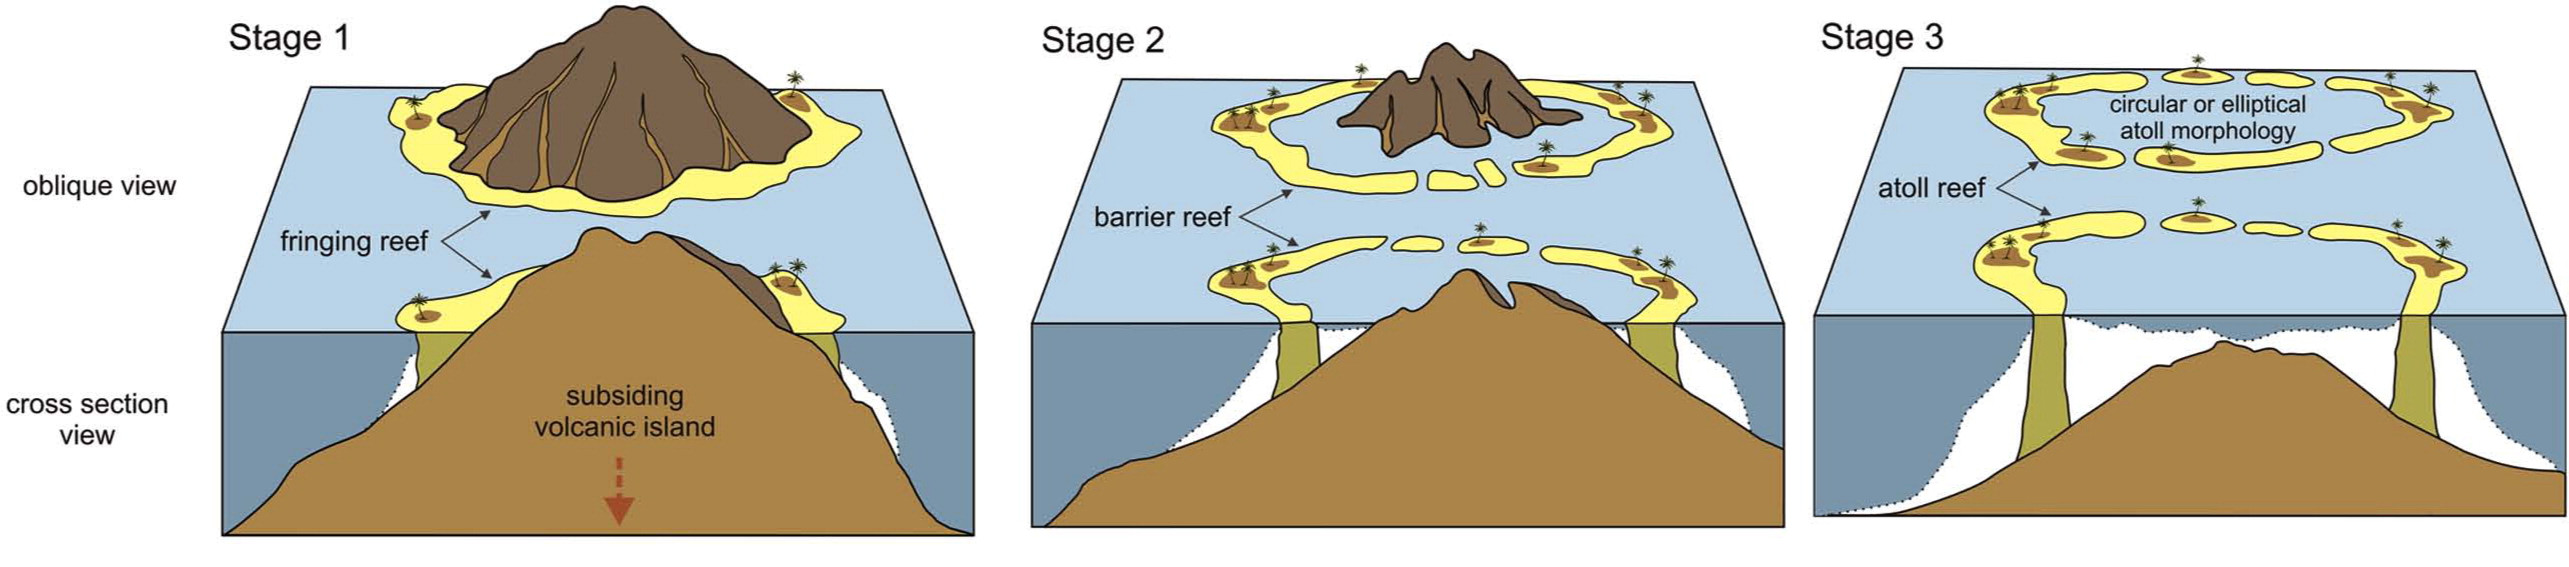
\includegraphics[width = \linewidth]{other_images/Drawings/Darwin_corals-color-Terry2012.jpg}
    \caption[Darwin's subsidence theory]{Coral colonies grow near sea level, forming a fringing reef (Stage 1). The island sinks slowly (subsidence); the coral reef continues its growth to keep living coral colonies in the photic zone. The sinking island increases the size of the lagoon, forming a barrier reef island (Stage 2). When the peak of the island is below the surface of the lagoon, an atoll is formed (Stage 3) \cite{Terry2013}.}
    \label{fig:coral-island-reef-growth}
\end{figure}

The formation of these islands involves processes at multiple scales, from the growth patterns of coral colonies to large-scale sediment transport, which are difficult to simulate directly. As a result, purely procedural or physics-based simulations fail to produce convincing or diverse coral reef island landscapes. On the other hand, deep learning methods are inoperable due to the extremely small amount of data, and the scarcity of high-resolution DEMs of these regions.

Despite advances in terrain generation, current methods struggle to support user-controlled design of specific island shapes and achieving realism without real data. Coral reef islands exemplify this gap: we lack datasets to directly train deep learning models, and purely procedural methods require expert tuning to mimic their features.

% To address these challenges, we use procedural generation as an initial step in our global pipeline. In this step we employ algorithmic rules to synthesise terrain features, allowing us to encode basic patterns of coral reef island formation. However, such algorithms are inherently rigid: they are tailored to a narrow family of shapes (in our case, radially organised and centred islands) and often rely on mathematical controls that are unintuitive for non-expert users. In our work, we use a procedural model not as the final solution, but as a means to efficiently create a large and diverse set of training examples for a learning-based model. Specifically, by adjusting procedural parameters, the procedural pipeline produces varied island scenarios. Each synthetic example is represented by a detailed terrain height field and a corresponding semantic label map that marks different regions, providing structured input-output pairs for the learning stage.

% We then train and deploy a conditional Generative Adversarial Network (cGAN) as the core of our method. A cGAN is a type of deep learning model that learns to generate realistic data based on an input condition or context. In our case, the cGAN takes as input the semantic label map of an island (a label layout indicating regions such as ocean, reef, beach, and mountain) generated by the procedural step and learns to produce a plausible island height field that matches this layout. By training on a large set of examples from the procedural generator, the cGAN captures subtle terrain features and variations unique to coral reef islands, going beyond what hard-coded procedural rules can achieve thanks to the application of data augmentation.

% Once the cGAN is trained on a sufficiently large and varied set of synthetic islands, it is used on its own to generate new island terrains. At this stage, our procedural generation module, only necessary to provide training data, is not required for creating new islands. Instead, a user provides a semantic map using digital drawing or another simple algorithm, and the cGAN generates a plausible island terrain accordingly. To summarise, our pipeline leverages procedural modelling to create a training dataset, and then relies on the learned cGAN model for the final generation of coral reef islands. In this way, we overcome the scarcity of real data by procedurally generating training examples, and overcome the rigidity of procedural rules through cGAN-based learning.

To address the scarcity of real-world coral reef island data and the limitations of purely procedural approaches, our pipeline combines procedural generation with a conditional Generative Adversarial Network (cGAN). First, a procedural model uses algorithmic rules to generate a large and diverse set of synthetic island examples, each consisting of a terrain height field and a corresponding semantic label map that identifies regions such as ocean, reef, lagoon, beach, and mountain. Although procedural methods efficiently encode basic formation patterns, they are inherently rigid, restricted to a narrow range of shapes, and often rely on unintuitive parameters. These synthetic examples are therefore used to train a cGAN, which learns to generate island height fields conditioned on semantic label maps. Through exposure to numerous procedurally generated examples and data augmentation, the cGAN captures complex terrain characteristics and variations that extend beyond handcrafted procedural rules. Once trained, the cGAN becomes the primary generation tool: users can provide semantic maps through digital drawing or other simple methods, and the network generates plausible coral reef island terrains without requiring the procedural model. In this way, procedural generation serves as a means of creating training data, while the cGAN provides a flexible and expressive solution for the final terrain generation process.



The key contributions of this paper are:
\begin{Itemize}
    \Item{} a novel sketch-based procedural algorithm for shaping island terrains from top and profile views,
    \Item{} the use of a deep learning model trained on synthetic data derived from procedural rules, acting as an abstraction layer that hides underlying complexity,
    \Item{} a demonstration that the cGAN approach tolerates imprecise, low-detail user input sketches, broadening usability, without the need for cutting-edge network architectures,
    \Item{} and an insight that procedural generation remains essential to produce training data in data-sparse domains, illustrated by the example of coral reef islands.
\end{Itemize}
These contributions collectively show a pathway for blending user-driven design with learning-based generation for terrain modelling.
